\section{Visibility of the lowest transfer energy}
\label{sec:visibility}

The lowest transfer excitation need not be created by a single spin.
We now show that its energy is nevertheless constrained by the lowest
mass seen by the spin field.  The odd eigenfunction from
Section~\ref{sec:parity} first detects a sign-cluster connection between
two rows.  Local circuits then attach a uniformly positive amount of
\emph{normalized} spin weight to that connection.

\begin{proposition}\label{vis:proposition}
Along the prescribed circumferences $w_k=M_0 2^k$,
\begin{equation}\label{vis:gap}
 \liminf_{k\to\infty}\;\liminf_{N\to\infty} e_N(w_k)\ge m_*.
\end{equation}
\end{proposition}

Throughout this section we work on the square torus of side $w=w_k$,
take $w$ sufficiently large, and put $d=\lfloor\sqrt w\rfloor$ in physical
units.  All fixed integer displacements below are lattice displacements,
since $a^{-1}=L^N$ is an integer.  Constants do not depend on $N$, $w$,
or translations of the specified test functions.

\subsection{From an odd eigenfunction to an open path}

Use the decomposition $q_x=(\cos\alpha_x\,z_x,\sin\alpha_x\,u_x)$
of Section~\ref{sec:parity}, where
$z_x=(\cos\vartheta_x,\sin\vartheta_x)$.  Conditional on $\alpha$, couple the Ising
signs $u_x$ to bonds $\eta_{xy}\in\{0,1\}$ by the Edwards--Sokal
construction~\cite{EdwardsSokal1988}, with couplings
\[
 J_{xy}(\alpha)=\beta_N\sin\alpha_x\sin\alpha_y.
\]
Given the full spin configuration, these bonds are independent: a bond
is closed when $u_x\ne u_y$, and otherwise is open with probability
$1-e^{-2J_{xy}(\alpha)}$.  In the reverse conditioning, given
$\alpha,\eta$, each connected component of open bonds receives an
independent fair sign.  These signs are also independent of the rotator
variables $z$.  We call the connected components \emph{sign clusters}.

The joint law of $(\alpha,\eta)$ is positively associated for the
coordinatewise order.  Indeed, the angle law is associated by
Lemma~\ref{par:association}.  Conditional on $\alpha$, the bond law has
weights proportional to
\[
 2^{k(\eta)}\prod_{xy:\,\eta_{xy}=1}
       \bigl(e^{2J_{xy}(\alpha)}-1\bigr),
\]
where $k(\eta)$ is the number of clusters.  Supermodularity of
$k(\eta)$ gives the FKG lattice condition, and increasing any coupling
increases this bond law stochastically~\cite{FKG1971}.  These facts hold
on the finite torus graph; zero couplings follow by continuity.
For increasing functions $f,g$ of $(\alpha,\eta)$, conditional
association gives
\[
 \E(fg\mid\alpha)\ge \E(f\mid\alpha)\E(g\mid\alpha).
\]
Both conditional means increase with $\alpha$, by the stochastic
monotonicity just noted.  A second application of association, now to
$\alpha$, proves the assertion.

\begin{lemma}\label{vis:row-lemma}
The probability that an open cluster meets both the row at time $0$
and the row at time $d$ satisfies
\begin{equation}\label{vis:row-connection}
 \Prob_{\mathrm{tor}}(0\longleftrightarrow d)
       \ge c\,e^{-(d+a)e_N(w)}.
\end{equation}
\end{lemma}

\begin{proof}
Suppress $N,w$ from the transfer notation.  Let $\psi$ be the real unit
$\tau$-eigenfunction furnished in Section~\ref{sec:parity}, where
$\tau=e^{-ae_N(w)}$, and choose color $3$ so that $\psi$ is odd under
its sign flip.  The row observable $F=\sgn\psi$, with $\sgn0=0$, is
bounded by one and has the same oddness.  Its torus correlation is
\[
 \E_{\mathrm{tor}}[F(0)F(d)]
 =\frac{\Tr\bigl(F T^{d/a}F T^{(w-d)/a}\bigr)}{R_{N,w}(w)}.
\]
Every summand in its eigenbasis expansion is nonnegative.  The summand
with $\psi$ on the segment of length $d$ and $\Omega$ on the other
segment is
\[
 \frac{e^{-de_N(w)}|\inner{\Omega}{F\psi}|^2}{R_{N,w}(w)}
 =\frac{e^{-de_N(w)}\inner{\Omega}{|\psi|}^2}{R_{N,w}(w)}
 \ge c\,e^{-(d+a)e_N(w)},
\]
by \eqref{par:overlap} and the uniform bound for $R_{N,w}(w)$ in
\eqref{tra:trace}.  Here $\tau/(1+\tau)\ge\tau/2$; in particular,
no bound on $ae_N(w)$ is required.

If no cluster meets both rows, flip the signs of every cluster meeting
the first row.  Conditional on $\alpha,z,\eta$, this preserves the law,
changes the sign of $F(0)$, and leaves $F(d)$ unchanged.  Thus the
conditional expectation of their product is zero off
$\{0\longleftrightarrow d\}$, and its absolute value is at most one
on that event.  The claimed probability bound follows.
\end{proof}

\subsection{Giving a cluster positive normalized weight}

A connection probability alone does not control the normalized field,
because the normalization $B_N$ varies with the cutoff.  We therefore
put $B_N$ into the cluster weights from the outset.  For nonnegative
smooth tests $h,h'$ supported in local torus charts, set
\begin{equation}\label{vis:weights}
 \begin{split}
 x_{\mathcal C}(h)&=B_Na^2\sum_{y\in\mathcal C}
                         h(y)\sin\alpha_y,\\
 S(h,h')&=\sum_{\mathcal C}x_{\mathcal C}(h)x_{\mathcal C}(h').
 \end{split}
\end{equation}
In this section $X_h=B_Na^2\sum_y h(y)q_y^3$.  Independent cluster
signs give the exact identity
\begin{equation}\label{vis:conditional-weight}
 \E(X_hX_{h'}\mid\alpha,\eta)=S(h,h').
\end{equation}
Moreover, $S(h,h')$ increases in $(\alpha,\eta)$: increasing an angle
increases every relevant sine factor, and merging two clusters adds
only nonnegative cross terms.

Fix a nonzero nonnegative $h\in C_c^\infty((-1,1)^2)$, and let
$h_s$ be its translate to a lattice center $s$.  Let $h'_s$ be the
translate to $s+10\mathbf e_t$, where $\mathbf e_t$ is the unit vector
in the time direction.  Tests are periodized on the torus.

\begin{lemma}\label{vis:weight-lemma}
There exist $\epsilon,c_0>0$ and fixed thresholds $N_0,w_0$ such that
for $N\ge N_0$, $w=w_k\ge w_0$, and every center $s$,
\begin{equation}\label{vis:positive-weight}
 \Prob_{\mathrm{tor}}\{S(h_s,h'_s)\ge\epsilon\}\ge c_0.
\end{equation}
\end{lemma}

\begin{proof}
By \eqref{vis:conditional-weight}, the expectation of $S(h_s,h'_s)$
is the corresponding normalized spin correlation.  Translation
invariance, plane moment convergence, and the strictly positive
continuum kernel of Lemma~\ref{inp:kernel} show that the cutoff plane
expectation is bounded below by a positive constant for all large
$N$.  Corollary~\ref{tra:moments} transfers
this lower bound to all sufficiently large $w$, uniformly in $N,s$.
Thus $\E_{\mathrm{tor}}S(h_s,h'_s)\ge c_1>0$.
Conditional Jensen and the uniform fourth moments give
\[
 \E_{\mathrm{tor}}S(h_s,h'_s)^2
 \le\E_{\mathrm{tor}}(X_{h_s}^2X_{h'_s}^2)\le C_1.
\]
The elementary second-moment inequality now yields
\[
 \Prob_{\mathrm{tor}}\{S(h_s,h'_s)\ge c_1/2\}
 \ge\frac{c_1^2}{4C_1}.
\]
All constants already include the field normalization, so they are
independent of the cutoff.
\end{proof}

\subsection{Circuits and the weighted connection estimate}

Write $Q_r(s)=s+[-r,r]^2$.  We next construct a connected open set
in $Q_6(s)\setminus\operatorname{int}Q_4(s)$ meeting every path from
$Q_1(s)$ to the exterior of $Q_6(s)$, with probability bounded below
uniformly.  Call such a set a \emph{barrier}.
The four strips are the translates and
quarter-turns of $[-6,6]\times[4,6]$.  A \emph{short-way} crossing
joins the sides at distance $2$; a \emph{long-way} crossing joins those
at distance $12$.

On the event in \eqref{vis:positive-weight}, some cluster joins
$Q_1(s)$ to $Q_1(s+10\mathbf e_t)$, hence exits $Q_6(s)$.
Follow such a path until its first hit of the boundary of $Q_6(s)$.
In a coordinate that reaches the boundary,
take the segment after its last visit to level $4$ with the relevant
sign.  This segment lies in one of the four strips and crosses it
short-way.  A union bound and square symmetry therefore give a fixed
positive lower bound for the short-way crossing probability of each
strip.

To obtain long-way crossings, we use the planar RSW theorem of
K\"ohler-Schindler and Tassion~\cite[Theorem~1, preprint version]{KohlerSchindlerTassion2023}.
In the notation $\mathcal H(m,n)$ for a horizontal crossing of
$[-m,m]\times[-n,n]$, its relevant assertion is that, for each
$r\ge1$, there is an increasing homeomorphism
$\Psi_r:[0,1]\to[0,1]$ such that
\begin{equation}\label{vis:rsw}
 \Prob\bigl(\mathcal H(rn,n)\bigr)
 \ge\Psi_r\!\left(\Prob\bigl(\mathcal H(n,rn)\bigr)\right)
\end{equation}
for a positively associated bond law on $\Z^2$ invariant under the
square-lattice symmetries.  We use $r=6$ and $n=a^{-1}$.

The law to which we apply this theorem is the \emph{cutoff plane} bond
law, obtained by sampling bonds conditional on the plane spins by the
same local edge rule.  It has the required square symmetries.
For a local bond event, its conditional probability given spins is a
bounded observable of the incident vertices, with supremum norm at
most one.  Consequently Proposition~\ref{tra:comparison} compares torus and
plane probabilities with error $Ce^{-cw}$, uniformly in the cutoff.
At fixed cutoff, taking the torus size to infinity also transfers
association to increasing cylinder events in the plane.
This suffices for association of arbitrary increasing Borel events:
compact subsets of an increasing event and its complement can be
separated by an increasing cylinder event, and inner regularity then
gives approximation in probability.  To see the separation, no
configuration in the first compact set is coordinatewise below one
in the second; compactness selects finitely many coordinates witnessing
all these failures of order.

Thus the short-way bound passes to the plane, \eqref{vis:rsw} gives a
uniform long-way bound there, and comparison passes that bound back
to all large tori.  The theorem requires neither a Markov property nor
association under changed spin boundary conditions.

Let $B_s$ be the increasing event that all four strips have long-way
crossings.  Positive association gives $\Prob_{\mathrm{tor}}(B_s)\ge c_2>0$.
Adjacent crossings meet: in their common $2$-by-$2$ corner square one
contains a horizontal crossing and the other a vertical crossing.
Their union is therefore connected.  Every path from $Q_1(s)$ to the
exterior of $Q_6(s)$ has a short-way crossing of one strip, by the
boundary-hit argument above, and hence intersects that strip's long-way
crossing.  Thus the four crossings form a barrier.  This is the
separating property of the circuit construction that we need, and
it holds in a single planar chart of the torus.

Set $H_s=h_s+h'_s$.  On
\[
 A_s=B_s\cap\{S(h_s,h'_s)\ge\epsilon\},
\]
every cluster contributing to $S(h_s,h'_s)$ meets the barrier and
therefore is the cluster containing it, say $\mathcal C_s$.  Hence
\[
 x_{\mathcal C_s}(h_s)x_{\mathcal C_s}(h'_s)\ge\epsilon,
 \qquad x_{\mathcal C_s}(H_s)\ge\sqrt\epsilon.
\]
The event $A_s$ is increasing and has probability at least $c_0c_2$.

Cover each row in Lemma~\ref{vis:row-lemma} by intervals of radius $1$
centered at integer spatial coordinates.  There are $O(w)$ intervals
per row.  For centers $s,t$ on the two rows, let $D_{st}$ be the event
that an open path joins their intervals.
For large $w$, the rings around $s$ and $t$ are disjoint.
On $D_{st}\cap A_s\cap A_t$, a connecting path meets both barriers,
so $\mathcal C_s$ and $\mathcal C_t$ are one cluster.  Its two
normalized weights give $S(H_s,H_t)\ge\epsilon$.  Association and
\eqref{vis:conditional-weight} therefore imply
\begin{equation}\label{vis:bridge}
 \E_{\mathrm{tor}}X_{H_s}X_{H_t}
 =\E_{\mathrm{tor}}S(H_s,H_t)
 \ge\epsilon(c_0c_2)^2\Prob_{\mathrm{tor}}(D_{st}).
\end{equation}
This is the promised conversion of an arbitrary connecting path into
a uniformly visible normalized correlation. Figure~\ref{fig:circuits}
shows the barrier construction and the merging of the two weighted
clusters.

\begin{figure}[tbp]
\centering
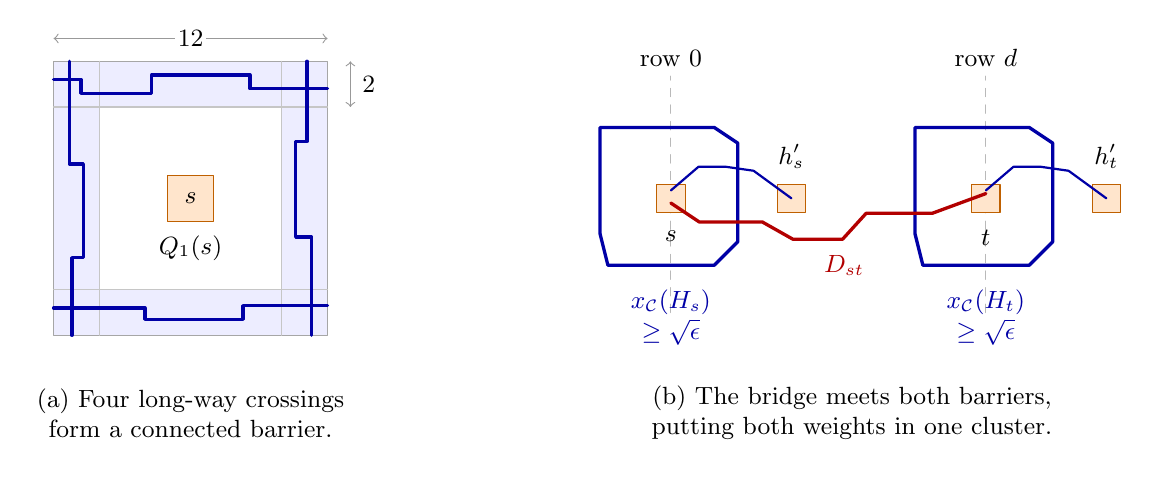
\begin{tikzpicture}[font=\small,line cap=round,line join=round]
 \begin{scope}[x=0.29cm,y=0.29cm]
  \fill[blue!7] (-6,-6) rectangle (6,6);
  \fill[white] (-4,-4) rectangle (4,4);
  \draw[gray!70] (-6,-6) rectangle (6,6);
  \draw[gray!70,dashed] (-4,-4) rectangle (4,4);
  \draw[gray!45] (-6,4)--(6,4) (-6,-4)--(6,-4)
                  (-4,-6)--(-4,6) (4,-6)--(4,6);
  \filldraw[fill=orange!20,draw=orange!75!black]
      (-1,-1) rectangle (1,1);
  \node at (0,0) {$s$};
  \node[anchor=north] at (0,-1.2) {$Q_1(s)$};
  \draw[blue!65!black,very thick]
     (-6,5.2)--(-4.8,5.2)--(-4.8,4.6)--(-1.7,4.6)
       --(-1.7,5.4)--(2.6,5.4)--(2.6,4.8)--(6,4.8);
  \draw[blue!65!black,very thick]
     (5.1,6)--(5.1,2.5)--(4.6,2.5)--(4.6,-1.7)
       --(5.3,-1.7)--(5.3,-6);
  \draw[blue!65!black,very thick]
     (6,-4.7)--(2.3,-4.7)--(2.3,-5.3)--(-2,-5.3)
       --(-2,-4.8)--(-6,-4.8);
  \draw[blue!65!black,very thick]
     (-5.2,-6)--(-5.2,-2.6)--(-4.7,-2.6)--(-4.7,1.5)
       --(-5.3,1.5)--(-5.3,6);
  \draw[<->,gray!80] (-6,7)--(6,7);
  \node[fill=white,inner sep=1pt] at (0,7) {$12$};
  \draw[<->,gray!80] (7,4)--(7,6);
  \node[anchor=west] at (7.1,5) {$2$};
  \node[align=center] at (0,-9.4)
     {(a) Four long-way crossings\\form a connected barrier.};
 \end{scope}
 \begin{scope}[shift={(6.1cm,0cm)},x=1cm,y=1cm]
  \draw[gray!55,dashed] (0,-1.45)--(0,1.55);
  \draw[gray!55,dashed] (4.0,-1.45)--(4.0,1.55);
  \node[above] at (0,1.55) {row $0$};
  \node[above] at (4,1.55) {row $d$};
  \foreach \u in {0,4} {
   \filldraw[fill=orange!20,draw=orange!75!black]
      (\u-0.18,-0.18) rectangle (\u+0.18,0.18);
   \filldraw[fill=orange!20,draw=orange!75!black]
      (\u+1.35,-0.18) rectangle (\u+1.71,0.18);
   \draw[blue!65!black,very thick]
      (\u-0.8,-0.85)--(\u+0.55,-0.85)--(\u+0.85,-0.55)
       --(\u+0.85,0.7)--(\u+0.55,0.9)--(\u-0.9,0.9)
       --(\u-0.9,-0.45)--cycle;
   \draw[blue!65!black,thick]
      (\u,0.1)--(\u+0.35,0.4)--(\u+0.7,0.4)
       --(\u+1.05,0.35)--(\u+1.53,0);
  }
  \draw[red!70!black,very thick]
    (0,-0.06)--(0.36,-0.3)--(1.16,-0.3)--(1.55,-0.52)
      --(2.18,-0.52)--(2.48,-0.19)--(3.32,-0.19)--(4,0.06);
  \node[below=3pt] at (0,-0.18) {$s$};
  \node[below=3pt] at (4,-0.18) {$t$};
  \node[above=2pt] at (1.53,0.18) {$h'_s$};
  \node[above=2pt] at (5.53,0.18) {$h'_t$};
  \node[red!70!black,below] at (2.2,-0.6) {$D_{st}$};
  \node[blue!65!black,below,align=center] at (0,-1.04)
      {$x_{\mathcal C}(H_s)$\\$\ge\sqrt\epsilon$};
  \node[blue!65!black,below,align=center] at (4,-1.04)
      {$x_{\mathcal C}(H_t)$\\$\ge\sqrt\epsilon$};
  \node[align=center] at (2.3,-2.72)
     {(b) The bridge meets both barriers,\\putting both weights in one cluster.};
 \end{scope}
\end{tikzpicture}
\caption{The geometric step in \eqref{vis:bridge}.
In (a), neighboring strip crossings meet in the corner squares.
In (b), on $A_s\cap A_t$, each barrier carries normalized weight
from the tests inside and outside it; any path in $D_{st}$ joins the
two barrier clusters.  Orange squares show test supports.  Panel (b)
is schematic: time runs horizontally and the distance between the
rings is compressed.}
\label{fig:circuits}
\end{figure}


\subsection{Taking the limits in the required order}

\begin{proof}[Proof of Proposition~\ref{vis:proposition}]
The union of the events $D_{st}$ contains
$\{0\longleftrightarrow d\}$.  Summing \eqref{vis:bridge} over the
$O(w^2)$ pairs and applying \eqref{vis:row-connection} gives
\[
 c\,e^{-(d+a)e_N(w)}
 \le\sum_{s,t}\E_{\mathrm{tor}}X_{H_s}X_{H_t}.
\]
Choose lifts with spatial center separation at most $w/2$.
The joint test supports then have spatial extent at most $w/2+O(1)$
and time extent at most $d+O(1)$, both less than $3w/4$ for large $w$.
The uniform moment comparison therefore replaces each torus
correlation by its cutoff plane value with error $Ce^{-cw}$.
For this \emph{fixed} $w$, there are only finitely many pairs of
centers, so plane moment convergence applies to all of them as
$N\to\infty$.  Their limiting correlations are bounded by
$Ce^{-m_*d}$: every pair of test supports has time separation at least
$d-O(1)$, and the kernel estimate \eqref{inp:decay} applies
to the fixed test shapes.  Consequently
\begin{equation}\label{vis:final-bound}
 \limsup_{N\to\infty}e^{-(d+a)e_N(w)}
 \le Cw^2\bigl(e^{-m_*d}+e^{-cw}\bigr).
\end{equation}

Write $L_w=\liminf_{N\to\infty}e_N(w)$.  If $L_w<\infty$, take a
subsequence on which $e_N(w)\to L_w$.  Along it $ae_N(w)\to0$, so
\eqref{vis:final-bound} yields
\[
 L_w\ge -\frac1d\log\!\left[
       Cw^2\bigl(e^{-m_*d}+e^{-cw}\bigr)\right].
\]
If $L_w=\infty$, the desired lower bound already holds.
Since $d=\lfloor\sqrt w\rfloor$, the displayed lower bound tends to
$m_*$ as $w=w_k\to\infty$, proving \eqref{vis:gap}.
\end{proof}

In particular, given $v<m_*$, every sufficiently large fixed $w_k$
satisfies $e_N(w_k)>v$ for all sufficiently large $N$, with the cutoff
threshold allowed to depend on $w_k$.  This order of quantifiers is
exactly what the finite doubling argument in
Section~\ref{sec:counting} will use.
